\section{Introduction and Motivation}
\label{sec:introduction}

This section describes the problem the Synchronic Web addresses and the design requirements that follow from that problem. It also states the trust assumptions and scope of the design.

\subsection{Durable Memory in a Mutable Web}

Most of what is written to the Web today will outlive the context in which it was created. A URL can remain stable while its content, operator, policy, software, and meaning all change. The database behind it usually carries richer detail, yet that detail travels poorly, because a recipient receives a representation while the operator retains its explanatory history. When the service closes or the relationship changes, evidence that seemed durable may collapse into screenshots, exports, and institutional memory. Version control, archives, local-first software, and user-controlled data each recover part of this continuity~\cite{Kleppmann2019local,Mansour2016solid}. Taken together, they outline a broader goal: a \glslink{resource}{resource} should remain identifiable across versions, interpretable beyond its current application, and citable from another institution's history. Corrections and disagreements should accumulate as later evidence rather than overwrite what came before, since a \glslink{record}{record} gains social value when several parties can preserve it from their own viewpoints and still compare what they retained. This need becomes acute wherever decisions outlive their supporting systems: scientific results, production records, public claims, personal identity, or an agent's sources and corrections. AI systems make the problem harder to ignore because they combine more context than a person can inspect directly~\cite{Lewis2020retrieval,Park2023generative,Anokhin2025arigraph,Gu2024hipporag}. The architectural question therefore reaches further than agents, to how independently operated systems share durable evidence while preserving their own authority over storage, policy, and interpretation.

\subsection{Independent Control and Shared Evidence}
\label{sec:control-evidence}

A plural Web needs both local control and structural connection, and the two pull in opposite directions. Local control lets each entity choose what to retain, expose, execute, and accept, whereas structural connection lets evidence cross institutional boundaries with its identity and historical context preserved. Together they create common evidence structures beneath independent roots, so evidence from separate local stores can be combined, and naming, ordering, and governance remain distributed among their operators. Reconciling them requires a precise account of who is trusted for what. The security model accordingly begins with an explicitly accepted commitment and separates four responsibilities:

\begin{itemize}
  \item \textbf{Structural integrity.} Collision-resistant hashing binds available material to the commitment, canonical encoding makes hashed and signed forms reproducible, and signatures associate a key with a committed \glslink{head}{head}.
  \item \textbf{Adversarial behavior.} Storage services, \glslink{journal}{journals}, intermediaries, and networks may omit, replay, delay, substitute, or selectively present material, while witnesses retain and compare signed views.
  \item \textbf{Operational assurance.} Replication and institutions sustain availability, disclosure policy and secure transport protect confidentiality, and domain evidence supports judgments about truth.
  \item \textbf{Local trust.} The client, evaluator, \glslink{integrity}{integrity} primitives, runtime configuration, operating-system boundary, and key store form the trusted base from which local policy interprets keys, \glslink{path}{paths}, and operations.
\end{itemize}

The compromise of a signing key shows how these responsibilities interact over time. Heads witnessed before key compromise remain evidence of the earlier history, while a compromised key can authorize later forks until bridged journals recognize the event. Key continuity follows predecessor-authorized transitions from the latest head each receiver retains (\cref{sec:bridge-histories}), which supports routine rotation without turning a journal into a permanent identity or making catastrophic recovery automatic. Loss or compromise of the accepted signing authority still requires an explicit governance decision.

\subsection{Portable State, Plural Trust}

The \glslink{synchronic-web}{Synchronic Web} lets state carry its own integrity evidence, history, and interpretation from one institution to another. Its compact thesis is \emph{\glslink{self-encoding}{self-encoding}, partially knowable, historically composable state with verifiable integrity}:

\begin{itemize}
  \item \textbf{Integrity} gives a logical state one stable identity.
  \item \textbf{Partial knowledge} lets observers retain different verifiable regions of that state.
  \item \textbf{History} orders successive states and composes selected remote heads into later local commits.
  \item \textbf{Self-encoding structure} carries definitions alongside the data they interpret.
\end{itemize}

Four terms recur throughout the paper. A \emph{journal} is the software an entity runs, together with all data that software persists, advancing a local history and supplying one viewpoint. A \emph{resource} is a path-addressed value or \glslink{object}{object} interpreted through that viewpoint. A \emph{\glslink{bridge}{bridge}} is a reciprocal relationship through which journals retain one another's verified \emph{heads}, the signed states each journal commits at successive history \glslink{index}{indexes}. A specialized client combines these layers so that applications can read resources, follow history, invoke objects, and traverse relationships through routine requests. \Cref{fig:journal-relative-web} shows this network. Each journal contains integrity-protected state and advances independently, while sparse bridges preserve remote heads and create cross-timeline ordering when those heads enter later commits. The highlighted journal supplies the operator viewpoint from which paths, identities, \glslink{route}{routes}, and policy acquire meaning. Trust therefore remains plural and divided among distinct checks. Structural verification answers whether evidence agrees with a commitment, signatures identify the key that authorized a head, historical routes connect that key to a journal known by the receiver, and \glslink{authorization}{authorization} applies the receiver's rules to the resulting \glslink{principal}{principal}. The architecture makes these checks composable and inspectable, but the final decision stays with the relying journal.

\begin{figure}[htbp]
  \centering
  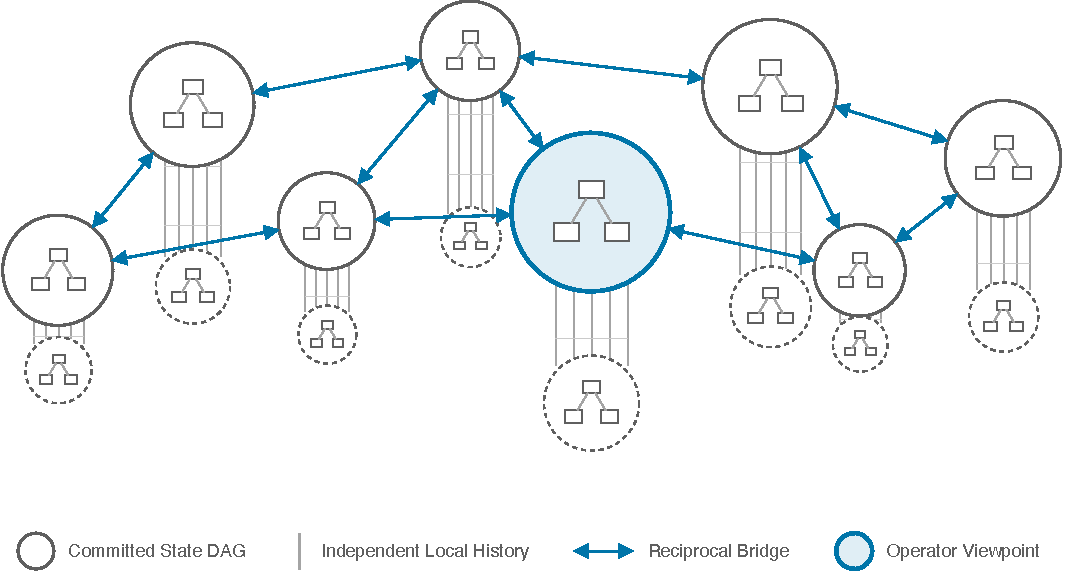
\includegraphics[scale=0.851]{figures/journal-relative-web.pdf}
  \caption{The Synchronic Web}
  \label{fig:journal-relative-web}
\end{figure}

\subsection{Scope and Lineage}

This paper is an architectural design and rationale. It describes the implemented integrity, history, object, and federation mechanisms and the assurance boundaries of their composition. The original Synchronic Web proposed a globally synchronized notary architecture~\cite{dinh2023synchronic}. The present design retains the name and broad aspiration but begins from independent journals, partially retained state, and sparse historical composition. Secure timelines and timeline entanglement supply the direct lineage for cross-history ordering~\cite{Maniatis2002timeline}. The architecture developed here asks what becomes possible when those histories carry everyday resources together with the definitions that interpret those resources.